\documentclass{ximera}  
\title{Sinusoidal Signals}  
\begin{document}  
\begin{abstract}  
Review of Sinusoidal Signals
\end{abstract}  

\chapter{Background Concepts Review}
\addcontentsline{toc}{chapter}{Background Concepts  Review}

\section{Sinusoidal Signals}
Sinusoidal signals are important  because all periodic signals can be represented with sinusoidal signals of different amplitudes and phases using Fourier series. 

Typical sinusoidal signal is shown in Figure \ref{sinusoid}. On the y-axis is the instantaneous value of the sinusoidal voltage and on the x-axis is time. Instantaneous values of voltage change from -1V to 1V with time. Sinusoidal signals can be characterized by the following parameters: peak amplitude, peak-to-peak, average, rms, period, time-delay and phase. Peak amplitude, peak-to-peak, average and rms values, are read on the y-axis in Figure \ref{sinusoid}, whereas period, time delay and phase are read on the x-axis.


\begin{enumerate}
\item Peak amplitude is measured on the y-axis as the length from the average value of the signal (in this case zero) to the maximum value of the signal (in this case 1). For signal shown in Figure \ref{sinusoid}, peak  amplitude has a constant value of $V_p=1$. Peak amplitude is NOT an instantaneous value of the signal, and it does not vary with  time. Sometimes amplitude and peak-amplitude are used interchangeably. Other times,  amplitude is used to denote an instantaneous value of the signal, and peak-amplitude is meant to denote the maximum value of amplitude. We will use amplitude to mean peak-amplitude. When we want to emphasize an instantaneous value of the signal, we will call it an instantaneous value.
\item Peak-to-peak is measured from the minimum value of the function (in this case -1) to the maximum value of the function (in this case 1).  For signal shown in Figure \ref{sinusoid}, peak-to-peak voltage has a constant value of  $V_{pp}=2$.
\item RMS or root-mean-square is defined as $v_{rms}=\frac{1}{T} \sqrt{\int_0^T v(t)^2 dt}$. For signal shown in Figure \ref{sinusoid}, and other sinusoidal signals of this form,  $v_{rms}=\frac{V_p}{\sqrt{2}}=\frac{1}{\sqrt{2}}=0.707$. Root mean square value  is important because it represents the equivalent amount of DC power.  
\item Average value $v_{ave1}=\frac{1}{T} \int_0^T v(t) dt$. For signal shown in Figure \ref{sinusoid}, average value is $V_{ave1}=0$ because the function has the same area under the function in the  positive and negative cycle. 
\item Period is measured on the x-axis as the length of one full cycle of the sinusoidal signal. For signal shown in Figure \ref{sinusoid}, this value is $period=T$
\item Time delay represents the lag (or lead) of one function with respect to another. For example, in Figure \ref{sinusoid}, function $ \cos(\omega t - 90^o)$ is time-delayed for $\tau = \frac{T}{4}$ with respect to $\cos (\omega t)$. To find the time delay for  a sinusoidal signal from its phase, we look at the way to represent the phase $90^o$ in terms of product of frequency and time. Since in the sinusoidal signal expression $\cos (\omega t + \Theta)$  phase $\Theta$ is added to $\omega t$ term, the phase has the same units as $\omega t$, and can be represented as the product of $\omega \tau = \theta$, $\tau = \frac{\theta}{\omega}$, where $\tau$ represents the time delay.
\item Phase of the signal is shown in Figure \ref{f11}(d)-(e).
\end{enumerate}

Review signals shown in Figure \ref{f11}. Signals in Figure \ref{f11}(a)-(b) are shown as a function of time, whereas signals in Figure \ref{f11}(c)-(d) are shown as a function of angle. See how are the graphs the same and how are they different. 

\begin{figure}[htbp]
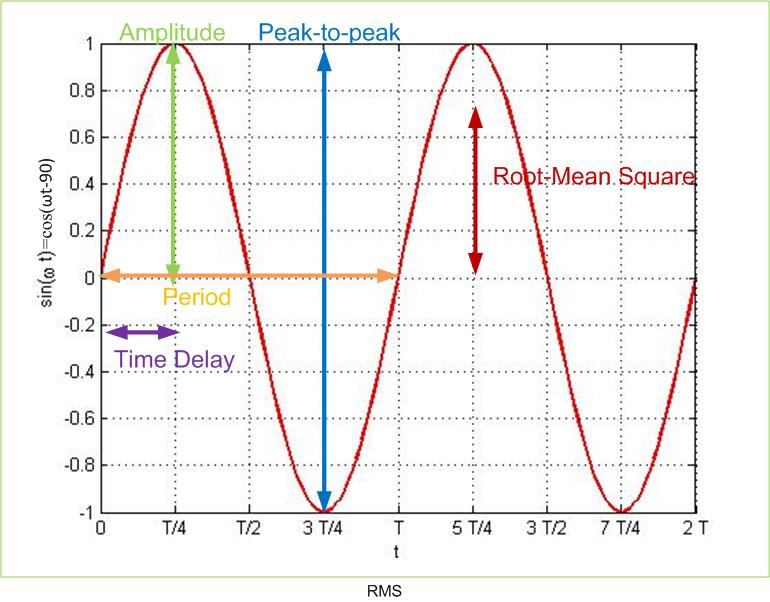
\includegraphics{sinusoid.jpg}
\end{figure} 





%\begin{figure}[htbp]
%\vspace*{-0.5cm}
%\begin{center}
%\subfigure[$sin ( \omega t)$]{
%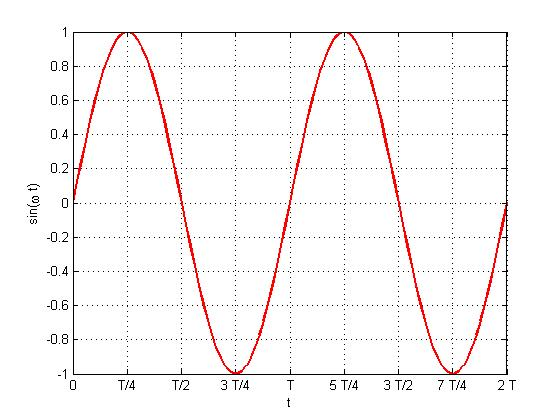
\includegraphics[scale=0.4]{jpg/cpef1.jpg}}
%\subfigure[ Sinusoidal signal shifted for time delay $-\frac{\pi/4}{\omega}$]{
%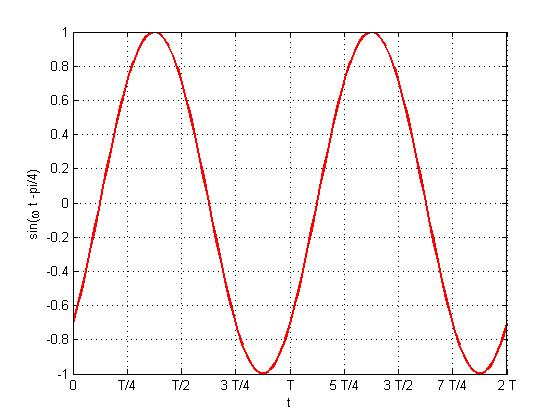
\includegraphics[scale=0.4]{jpg/cpef2.jpg}}
%\subfigure[Sinusoidal signal as a function of angle $\omega t$]{
%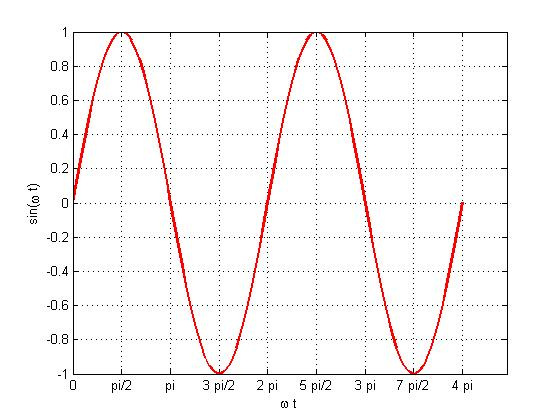
\includegraphics[scale=0.4]{jpg/cpef3.jpg}}
%\subfigure[Sinusoidal signal as a function of angle $\omega t$ with a phase shift of $-\pi/4$]{
%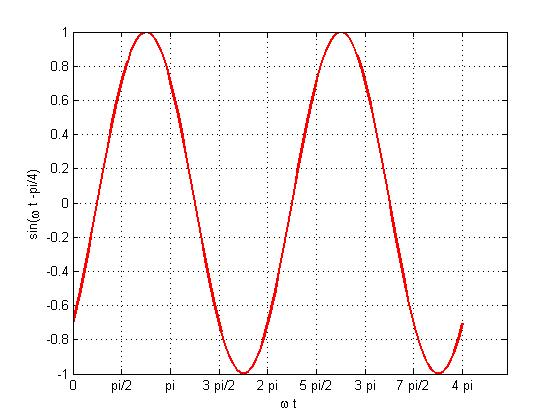
\includegraphics[scale=0.4]{jpg/cpef4.jpg}}
%\subfigure[Sinusoidal signal as a function of angle $\omega t$ with a phase shift of $+\pi/4$]{
%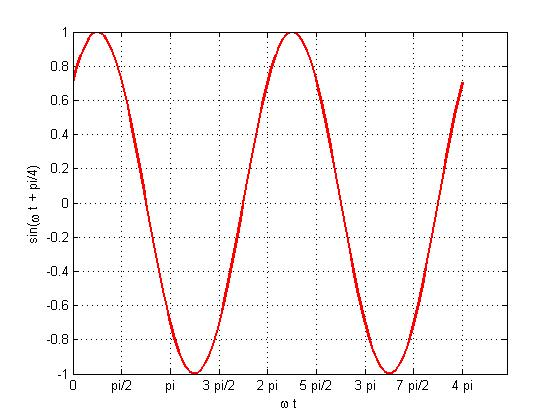
\includegraphics[scale=0.4]{jpg/cpef5.jpg}}
%\strut\psfig{figure=cpef1.ps,width=10cm}
%\end{center}
%\caption{\label{f11} Sinusoidal signal as a function of time (a)-(b) and angle (c)-(e).}
%\end{figure}



%\begin{figure}[htbp]
%\vspace*{-0.5cm}
%\begin{center}

%\subfigure[Sinusoidal signals of different frequencies $sin ( \omega t)$]{
%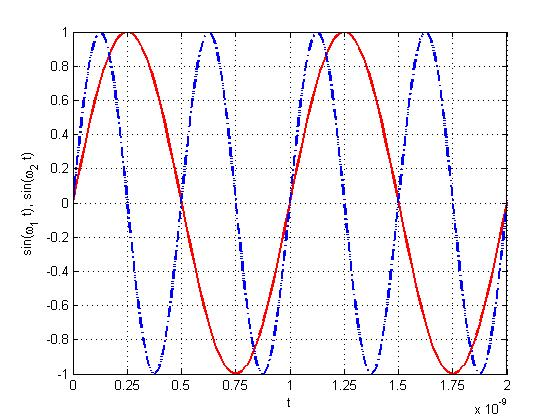
\includegraphics[scale=0.4]{jpg/cpef6.jpg}}
%\subfigure[Sinusoidal signals of different amplitudes $sin ( \omega t)$]{
%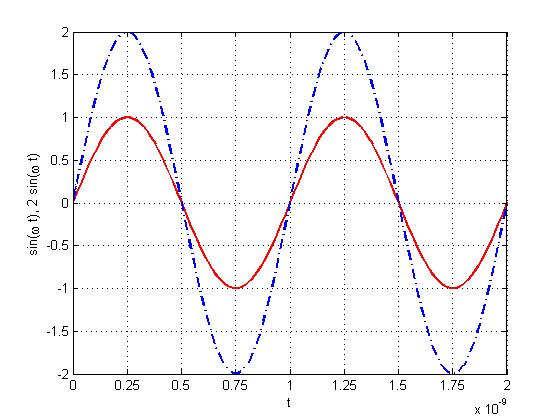
\includegraphics[scale=0.4]{jpg/cpef7.jpg}}
%%\strut\psfig{figure=cpef1.ps,width=10cm}
%\end{center}
%\caption{\label{f2} Comparison of sinusoidal signals.}
%\end{figure}













                                                                   



                                       




                                    














\maketitle    
  Calculate.
\begin{question}  
$3\times 2 = \answer{6}$  
\end{question} 
\end{document} 
